\documentclass{iopjournal}
\usepackage{amssymb,amsmath,booktabs,array,multirow,adjustbox,makecell,microtype,placeins,ragged2e}
\usepackage[round]{natbib}
\hypersetup{hidelinks,pdftitle={Supplementary material: Subject-independent forearm sEMG electrode reduction with cross-fitted attribution and non-inferiority testing},pdfauthor={Minh-Tri Ta, Hoang-Khang Phan, Le-Giang Tran}}\AtBeginDocument{\justifying}


\newcommand{\GRABMyoParticipants}{43}
\newcommand{\GRABMyoSessions}{3}
\newcommand{\GRABMyoGestures}{17}
\newcommand{\GRABMyoActiveGestures}{16}
\newcommand{\GRABMyoWindows}{598{,}689}
\newcommand{\GRABMyoRecords}{15{,}351}
\newcommand{\GRABMyoRecordsFailed}{0}
\newcommand{\GRABMyoAgeMean}{26.4}
\newcommand{\GRABMyoAgeSD}{2.9}
\newcommand{\GRABMyoMale}{23}
\newcommand{\GRABMyoFemale}{20}
\newcommand{\GRABMyoCircMean}{24.1}
\newcommand{\GRABMyoCircSD}{2.3}
\newcommand{\GRABMyoArcSpacing}{3.0}
\newcommand{\GRABMyoActiveWindows}{563{,}472}
\newcommand{\FoldTrainingWindows}{550{,}368}
\newcommand{\TestWindowsPerParticipant}{13{,}104}
\newcommand{\DBFiveSubjects}{10}
\newcommand{\DBFiveAgeMean}{28.0}
\newcommand{\DBFiveAgeSD}{4.0}
\newcommand{\DBFiveMale}{8}
\newcommand{\DBFiveFemale}{2}
\newcommand{\DBFiveWindows}{21{,}089}
\newcommand{\GRABMyoFilesVerified}{30{,}715}
\newcommand{\FullRF}{0.502}
\newcommand{\FullRFLCB}{0.475}
\newcommand{\FullRFUCB}{0.528}
\newcommand{\FullRFSD}{0.090}
\newcommand{\FullRFMin}{0.346}
\newcommand{\FullRFMax}{0.670}
\newcommand{\FullSVM}{0.538}
\newcommand{\FullSVMLCB}{0.513}
\newcommand{\FullSVMUCB}{0.562}
\newcommand{\FullSVMSD}{0.085}
\newcommand{\FullSVMMin}{0.383}
\newcommand{\FullSVMMax}{0.718}
\newcommand{\FullXGB}{0.542}
\newcommand{\FullXGBLCB}{0.517}
\newcommand{\FullXGBUCB}{0.567}
\newcommand{\FullXGBSD}{0.085}
\newcommand{\FullXGBMin}{0.385}
\newcommand{\FullXGBMax}{0.702}
\newcommand{\KStarMarginPtOne}{14}
\newcommand{\KStarMarginPtTwo}{12}
\newcommand{\KStarMarginPtThree}{11}
\newcommand{\KStar}{12}
\newcommand{\KStarReductionPct}{25}
\newcommand{\SVMvsRFDiff}{+0.0362}
\newcommand{\SVMvsRFLCB}{+0.0284}
\newcommand{\SVMvsRFUCB}{+0.0444}
\newcommand{\SVMvsRFW}{15.0}
\newcommand{\SVMvsRFP}{< 0.001}
\newcommand{\SVMvsRFR}{+0.97}
\newcommand{\XGBvsRFDiff}{+0.0408}
\newcommand{\XGBvsRFLCB}{+0.0340}
\newcommand{\XGBvsRFUCB}{+0.0475}
\newcommand{\XGBvsRFW}{10.0}
\newcommand{\XGBvsRFP}{< 0.001}
\newcommand{\XGBvsRFR}{+0.98}
\newcommand{\XGBvsSVMDiff}{+0.0045}
\newcommand{\XGBvsSVMLCB}{-0.0015}
\newcommand{\XGBvsSVMUCB}{+0.0107}
\newcommand{\XGBvsSVMW}{354.0}
\newcommand{\XGBvsSVMP}{= 0.154}
\newcommand{\XGBvsSVMR}{+0.25}
\newcommand{\SVMCalibTwentyK}{0.555}
\newcommand{\SVMCalibFortyK}{0.591}
\newcommand{\CurveKSixteen}{0.541}
\newcommand{\CurveKSixteenSD}{0.084}
\newcommand{\CurveKFourteen}{0.535}
\newcommand{\CurveKFourteenSD}{0.083}
\newcommand{\DeltaKFourteen}{-0.0060}
\newcommand{\DeltaKFourteenLCB}{-0.0081}
\newcommand{\DeltaKFourteenUCB}{-0.0039}
\newcommand{\CurveKThirteen}{0.530}
\newcommand{\CurveKThirteenSD}{0.083}
\newcommand{\DeltaKThirteen}{-0.0109}
\newcommand{\DeltaKThirteenLCB}{-0.0133}
\newcommand{\DeltaKThirteenUCB}{-0.0085}
\newcommand{\CurveKTwelve}{0.528}
\newcommand{\CurveKTwelveSD}{0.084}
\newcommand{\DeltaKTwelve}{-0.0133}
\newcommand{\DeltaKTwelveLCB}{-0.0160}
\newcommand{\DeltaKTwelveUCB}{-0.0106}
\newcommand{\CurveKEleven}{0.521}
\newcommand{\CurveKElevenSD}{0.084}
\newcommand{\DeltaKEleven}{-0.0204}
\newcommand{\DeltaKElevenLCB}{-0.0246}
\newcommand{\DeltaKElevenUCB}{-0.0162}
\newcommand{\CurveKTen}{0.515}
\newcommand{\CurveKTenSD}{0.083}
\newcommand{\DeltaKTen}{-0.0259}
\newcommand{\DeltaKTenLCB}{-0.0311}
\newcommand{\DeltaKTenUCB}{-0.0205}
\newcommand{\CurveKEight}{0.505}
\newcommand{\CurveKEightSD}{0.085}
\newcommand{\DeltaKEight}{-0.0366}
\newcommand{\DeltaKEightLCB}{-0.0440}
\newcommand{\DeltaKEightUCB}{-0.0289}
\newcommand{\CurveKSix}{0.480}
\newcommand{\CurveKSixSD}{0.084}
\newcommand{\DeltaKSix}{-0.0610}
\newcommand{\DeltaKSixLCB}{-0.0713}
\newcommand{\DeltaKSixUCB}{-0.0507}
\newcommand{\CurveKFour}{0.397}
\newcommand{\CurveKFourSD}{0.071}
\newcommand{\DeltaKFour}{-0.1444}
\newcommand{\DeltaKFourLCB}{-0.1590}
\newcommand{\DeltaKFourUCB}{-0.1306}
\newcommand{\CurveKTwo}{0.299}
\newcommand{\CurveKTwoSD}{0.057}
\newcommand{\DeltaKTwo}{-0.2420}
\newcommand{\DeltaKTwoLCB}{-0.2603}
\newcommand{\DeltaKTwoUCB}{-0.2230}
\newcommand{\CurveKOne}{0.181}
\newcommand{\CurveKOneSD}{0.040}
\newcommand{\DeltaKOne}{-0.3603}
\newcommand{\DeltaKOneLCB}{-0.3832}
\newcommand{\DeltaKOneUCB}{-0.3369}
\newcommand{\CurveTrainWindows}{200{,}000}
\newcommand{\LambdaCurveMaxSpread}{0.0040}
\newcommand{\TopFourSet}{4, 6, 7, 14}
\newcommand{\TopFourFolds}{36}
\newcommand{\DroppedFourSet}{9, 11, 12, 16}
\newcommand{\DroppedFourFolds}{43}
\newcommand{\TopFourShare}{34.0}
\newcommand{\BottomEightShare}{39.6}
\newcommand{\UOverAMedian}{2.4}
\newcommand{\UOverAMax}{9.4}
\newcommand{\TopTwelveDiffersLambdaPtTwoFive}{0}
\newcommand{\TopTwelveDiffersLambdaPtFive}{0}
\newcommand{\TopTwelveDiffersLambdaOne}{1}
\newcommand{\HTwoKFourDiff}{+0.0172}
\newcommand{\HTwoKFourLCB}{+0.0071}
\newcommand{\HTwoKFourUCB}{+0.0274}
\newcommand{\HTwoKFourP}{= 0.007}
\newcommand{\HTwoKFourR}{+0.50}
\newcommand{\HTwoKSixDiff}{+0.0370}
\newcommand{\HTwoKSixLCB}{+0.0286}
\newcommand{\HTwoKSixUCB}{+0.0452}
\newcommand{\HTwoKSixP}{< 0.001}
\newcommand{\HTwoKSixR}{+0.92}
\newcommand{\HTwoKEightDiff}{+0.0243}
\newcommand{\HTwoKEightLCB}{+0.0176}
\newcommand{\HTwoKEightUCB}{+0.0308}
\newcommand{\HTwoKEightP}{< 0.001}
\newcommand{\HTwoKEightR}{+0.86}
\newcommand{\HTwoKTwelveDiff}{+0.0074}
\newcommand{\HTwoKTwelveLCB}{+0.0046}
\newcommand{\HTwoKTwelveUCB}{+0.0103}
\newcommand{\HTwoKTwelveP}{< 0.001}
\newcommand{\HTwoKTwelveR}{+0.71}
\newcommand{\HTwoAllSig}{yes}
\newcommand{\PctKFour}{65}
\newcommand{\PctKAboveNinetyFiveFour}{3}
\newcommand{\PctKSix}{89}
\newcommand{\PctKAboveNinetyFiveSix}{11}
\newcommand{\PctKEight}{82}
\newcommand{\PctKAboveNinetyFiveEight}{6}
\newcommand{\PctKTwelve}{66}
\newcommand{\PctKAboveNinetyFiveTwelve}{1}
\newcommand{\VSPermKFourDiff}{-0.0018}
\newcommand{\VSPermKFourP}{= 0.678}
\newcommand{\VSGeomKFourDiff}{-0.0005}
\newcommand{\VSGeomKFourP}{= 0.986}
\newcommand{\VSMiKFourDiff}{+0.1031}
\newcommand{\VSMiKFourP}{< 0.001}
\newcommand{\VSPermKSixDiff}{+0.0126}
\newcommand{\VSPermKSixP}{= 0.009}
\newcommand{\VSGeomKSixDiff}{+0.0341}
\newcommand{\VSGeomKSixP}{< 0.001}
\newcommand{\VSMiKSixDiff}{+0.0934}
\newcommand{\VSMiKSixP}{< 0.001}
\newcommand{\VSPermKEightDiff}{+0.0033}
\newcommand{\VSPermKEightP}{= 0.069}
\newcommand{\VSGeomKEightDiff}{+0.0047}
\newcommand{\VSGeomKEightP}{= 0.267}
\newcommand{\VSMiKEightDiff}{+0.0737}
\newcommand{\VSMiKEightP}{< 0.001}
\newcommand{\VSPermKTwelveDiff}{+0.0001}
\newcommand{\VSPermKTwelveP}{= 0.995}
\newcommand{\VSGeomKTwelveDiff}{+0.0070}
\newcommand{\VSGeomKTwelveP}{= 0.058}
\newcommand{\VSMiKTwelveDiff}{+0.0051}
\newcommand{\VSMiKTwelveP}{= 0.007}
\newcommand{\HThreeMaxAbsDiff}{0.0015}
\newcommand{\HThreeNSig}{0}
\newcommand{\HThreeNTests}{12}
\newcommand{\HThreeMinP}{= 0.216}
\newcommand{\HThreeMinTied}{36}
\newcommand{\FaithProtocolCells}{172}
\newcommand{\FaithProtocolMeanDiff}{0.0014}
\newcommand{\FaithProtocolMaxDiff}{0.0084}
\newcommand{\FaithTopKTwo}{0.263}
\newcommand{\FaithBottomKTwo}{0.292}
\newcommand{\FaithTopKFour}{0.351}
\newcommand{\FaithRandomKFour}{0.366}
\newcommand{\FaithBottomKFour}{0.382}
\newcommand{\FaithTopKSix}{0.376}
\newcommand{\FaithRandomKSix}{0.416}
\newcommand{\FaithBottomKSix}{0.454}
\newcommand{\FaithTopKEight}{0.408}
\newcommand{\FaithRandomKEight}{0.445}
\newcommand{\FaithBottomKEight}{0.469}
\newcommand{\FaithTopKTen}{0.445}
\newcommand{\FaithBottomKTen}{0.475}
\newcommand{\FaithTopKTwelve}{0.455}
\newcommand{\FaithRandomKTwelve}{0.478}
\newcommand{\FaithBottomKTwelve}{0.485}
\newcommand{\FaithTopKFourteen}{0.487}
\newcommand{\FaithBottomKFourteen}{0.491}
\newcommand{\FaithTBKTwoDiff}{-0.0297}
\newcommand{\FaithTBKTwoLCB}{-0.0419}
\newcommand{\FaithTBKTwoUCB}{-0.0166}
\newcommand{\FaithTBKTwoP}{< 0.001}
\newcommand{\FaithTBKFourDiff}{-0.0314}
\newcommand{\FaithTBKFourLCB}{-0.0447}
\newcommand{\FaithTBKFourUCB}{-0.0177}
\newcommand{\FaithTBKFourP}{< 0.001}
\newcommand{\FaithTRKFourDiff}{-0.0151}
\newcommand{\FaithTRKFourLCB}{-0.0239}
\newcommand{\FaithTRKFourUCB}{-0.0061}
\newcommand{\FaithTRKFourP}{= 0.010}
\newcommand{\FaithRBKFourDiff}{-0.0163}
\newcommand{\FaithRBKFourLCB}{-0.0265}
\newcommand{\FaithRBKFourUCB}{-0.0061}
\newcommand{\FaithRBKFourP}{= 0.013}
\newcommand{\FaithTBKSixDiff}{-0.0775}
\newcommand{\FaithTBKSixLCB}{-0.0921}
\newcommand{\FaithTBKSixUCB}{-0.0627}
\newcommand{\FaithTBKSixP}{< 0.001}
\newcommand{\FaithTRKSixDiff}{-0.0398}
\newcommand{\FaithTRKSixLCB}{-0.0487}
\newcommand{\FaithTRKSixUCB}{-0.0307}
\newcommand{\FaithTRKSixP}{< 0.001}
\newcommand{\FaithRBKSixDiff}{-0.0377}
\newcommand{\FaithRBKSixLCB}{-0.0459}
\newcommand{\FaithRBKSixUCB}{-0.0293}
\newcommand{\FaithRBKSixP}{< 0.001}
\newcommand{\FaithTBKEightDiff}{-0.0618}
\newcommand{\FaithTBKEightLCB}{-0.0772}
\newcommand{\FaithTBKEightUCB}{-0.0461}
\newcommand{\FaithTBKEightP}{< 0.001}
\newcommand{\FaithTRKEightDiff}{-0.0377}
\newcommand{\FaithTRKEightLCB}{-0.0476}
\newcommand{\FaithTRKEightUCB}{-0.0273}
\newcommand{\FaithTRKEightP}{< 0.001}
\newcommand{\FaithRBKEightDiff}{-0.0242}
\newcommand{\FaithRBKEightLCB}{-0.0309}
\newcommand{\FaithRBKEightUCB}{-0.0172}
\newcommand{\FaithRBKEightP}{< 0.001}
\newcommand{\FaithTBKTenDiff}{-0.0297}
\newcommand{\FaithTBKTenLCB}{-0.0399}
\newcommand{\FaithTBKTenUCB}{-0.0188}
\newcommand{\FaithTBKTenP}{< 0.001}
\newcommand{\FaithTBKTwelveDiff}{-0.0302}
\newcommand{\FaithTBKTwelveLCB}{-0.0385}
\newcommand{\FaithTBKTwelveUCB}{-0.0218}
\newcommand{\FaithTBKTwelveP}{< 0.001}
\newcommand{\FaithTRKTwelveDiff}{-0.0228}
\newcommand{\FaithTRKTwelveLCB}{-0.0296}
\newcommand{\FaithTRKTwelveUCB}{-0.0158}
\newcommand{\FaithTRKTwelveP}{< 0.001}
\newcommand{\FaithRBKTwelveDiff}{-0.0074}
\newcommand{\FaithRBKTwelveLCB}{-0.0101}
\newcommand{\FaithRBKTwelveUCB}{-0.0046}
\newcommand{\FaithRBKTwelveP}{< 0.001}
\newcommand{\FaithTBKFourteenDiff}{-0.0038}
\newcommand{\FaithTBKFourteenLCB}{-0.0084}
\newcommand{\FaithTBKFourteenUCB}{+0.0009}
\newcommand{\FaithTBKFourteenP}{= 0.150}
\newcommand{\FaithNTests}{15}
\newcommand{\FaithNSig}{14}
\newcommand{\FaithTBAllSig}{no}
\newcommand{\StabSubjPairs}{903}
\newcommand{\StabSubjRho}{0.927}
\newcommand{\StabSubjRhoSD}{0.038}
\newcommand{\StabSubjJacFour}{0.752}
\newcommand{\StabSubjJacSix}{0.905}
\newcommand{\StabSubjJacEight}{0.803}
\newcommand{\StabInnerPairs}{430}
\newcommand{\StabInnerRho}{0.948}
\newcommand{\StabInnerRhoSD}{0.021}
\newcommand{\StabInnerJacFour}{0.816}
\newcommand{\StabInnerJacSix}{0.992}
\newcommand{\StabInnerJacEight}{0.838}
\newcommand{\StabOuterPairs}{903}
\newcommand{\StabOuterRho}{0.987}
\newcommand{\StabOuterRhoSD}{0.008}
\newcommand{\StabOuterJacFour}{0.888}
\newcommand{\StabOuterJacSix}{1.000}
\newcommand{\StabOuterJacEight}{0.923}
\newcommand{\CSOneSOne}{0.492}
\newcommand{\CSOneSOneSD}{0.101}
\newcommand{\CSOneSOneTrain}{183{,}456}
\newcommand{\CSOneSTwo}{0.528}
\newcommand{\CSOneSTwoSD}{0.088}
\newcommand{\CSOneSTwoTrain}{183{,}456}
\newcommand{\CSOneSThree}{0.510}
\newcommand{\CSOneSThreeSD}{0.090}
\newcommand{\CSOneSThreeTrain}{183{,}456}
\newcommand{\CSTwoSThree}{0.530}
\newcommand{\CSTwoSThreeSD}{0.095}
\newcommand{\CSTwoSThreeTrain}{366{,}912}
\newcommand{\CSSTwoVsSOneDiff}{+0.0355}
\newcommand{\CSSTwoVsSOneLCB}{+0.0091}
\newcommand{\CSSTwoVsSOneUCB}{+0.0621}
\newcommand{\CSSTwoVsSOneW}{287.0}
\newcommand{\CSSTwoVsSOneP}{= 0.024}
\newcommand{\CSSThreeVsSOneDiff}{+0.0172}
\newcommand{\CSSThreeVsSOneLCB}{-0.0038}
\newcommand{\CSSThreeVsSOneUCB}{+0.0391}
\newcommand{\CSSThreeVsSOneW}{381.0}
\newcommand{\CSSThreeVsSOneP}{= 0.272}
\newcommand{\CSTwoVsOneDiff}{+0.0210}
\newcommand{\CSTwoVsOneLCB}{+0.0146}
\newcommand{\CSTwoVsOneUCB}{+0.0274}
\newcommand{\CSTwoVsOneW}{77.0}
\newcommand{\CSTwoVsOneP}{< 0.001}
\newcommand{\DBFiveFull}{0.281}
\newcommand{\DBFiveFullSD}{0.099}
\newcommand{\DBFiveFullMin}{0.096}
\newcommand{\DBFiveFullMax}{0.386}
\newcommand{\DBFiveKSixteen}{0.281}
\newcommand{\DBFiveKSixteenSD}{0.099}
\newcommand{\DBFiveKTwelve}{0.268}
\newcommand{\DBFiveKTwelveSD}{0.092}
\newcommand{\DBFiveKEight}{0.252}
\newcommand{\DBFiveKEightSD}{0.068}
\newcommand{\DBFiveKFour}{0.180}
\newcommand{\DBFiveKFourSD}{0.026}
\newcommand{\DBFiveDeltaKEleven}{-0.0211}
\newcommand{\DBFiveDeltaKElevenLCB}{-0.03412}
\newcommand{\DBFiveDeltaKTwelve}{-0.0126}
\newcommand{\DBFiveDeltaKTwelveLCB}{-0.01999}
\newcommand{\DBFiveDeltaKThirteen}{-0.0143}
\newcommand{\DBFiveDeltaKThirteenLCB}{-0.03119}
\newcommand{\DBFiveDeltaKFourteen}{-0.0119}
\newcommand{\DBFiveDeltaKFourteenLCB}{-0.02744}
\newcommand{\DBFiveDeltaKFifteen}{-0.0108}
\newcommand{\DBFiveDeltaKFifteenLCB}{-0.02377}
\newcommand{\DBFiveKStarMarginPtOne}{none}
\newcommand{\DBFiveKStarMarginPtTwo}{12}
\newcommand{\DBFiveKStarMarginPtThree}{12}
\newcommand{\DBFiveNIPassing}{12}
\newcommand{\DBFiveMonteCarloFrac}{95.5}
\newcommand{\DBFiveMonteCarloN}{200}
\newcommand{\DBFiveMonteCarloHits}{191}
\newcommand{\DBFiveMonteCarloLCBMin}{-0.0201}
\newcommand{\DBFiveMonteCarloLCBMax}{-0.0195}
\newcommand{\BipFull}{0.478}
\newcommand{\BipFullSD}{0.089}
\newcommand{\BipKOne}{0.174}
\newcommand{\BipKOneSD}{0.044}
\newcommand{\BipKTwo}{0.240}
\newcommand{\BipKTwoSD}{0.049}
\newcommand{\BipKThree}{0.310}
\newcommand{\BipKThreeSD}{0.070}
\newcommand{\BipKFour}{0.356}
\newcommand{\BipKFourSD}{0.080}
\newcommand{\BipKFive}{0.405}
\newcommand{\BipKFiveSD}{0.085}
\newcommand{\BipKSix}{0.442}
\newcommand{\BipKSixSD}{0.086}
\newcommand{\BipKSeven}{0.464}
\newcommand{\BipKSevenSD}{0.085}
\newcommand{\BipKEight}{0.480}
\newcommand{\BipKEightSD}{0.089}
\newcommand{\BipDeltaKOne}{-0.3052}
\newcommand{\BipDeltaKOneLCB}{-0.3298}
\newcommand{\BipDeltaKTwo}{-0.2399}
\newcommand{\BipDeltaKTwoLCB}{-0.2615}
\newcommand{\BipDeltaKThree}{-0.1697}
\newcommand{\BipDeltaKThreeLCB}{-0.1852}
\newcommand{\BipDeltaKFour}{-0.1240}
\newcommand{\BipDeltaKFourLCB}{-0.1392}
\newcommand{\BipDeltaKFive}{-0.0742}
\newcommand{\BipDeltaKFiveLCB}{-0.0845}
\newcommand{\BipDeltaKSix}{-0.0375}
\newcommand{\BipDeltaKSixLCB}{-0.0451}
\newcommand{\BipDeltaKSeven}{-0.0158}
\newcommand{\BipDeltaKSevenLCB}{-0.0203}
\newcommand{\BipKStarMarginPtOne}{none}
\newcommand{\BipKStarMarginPtTwo}{none}
\newcommand{\BipKStarMarginPtThree}{7}
\newcommand{\BipolarMonteCarloFracSeven}{0}
\newcommand{\BipolarMonteCarloHitsSeven}{0}
\newcommand{\BipolarMonteCarloN}{200}
\newcommand{\BipolarMonteCarloLCBMaxSeven}{-0.0203}
\newcommand{\BipolarMonteCarloLCBMinSeven}{-0.0207}
\newcommand{\BipCurveRefK}{0.480}
\newcommand{\BipTopThreeSet}{5, 6, 7}
\newcommand{\BipTopThreeFolds}{30}
\newcommand{\FixedDev}{22}
\newcommand{\FixedTest}{21}
\newcommand{\FixedChannels}{1, 2, 4, 5, 6, 7, 8, 10, 13, 14, 15, 16}
\newcommand{\FixedDropped}{3, 9, 11, 12}
\newcommand{\FixedFull}{0.522}
\newcommand{\FixedTwelve}{0.510}
\newcommand{\FixedDiff}{-0.0124}
\newcommand{\FixedLCB}{-0.0179}
\newcommand{\FixedUCB}{-0.0077}
\newcommand{\FixedLamZeroSame}{yes}
\newcommand{\FixedNLambdaSameOrig}{4}
\newcommand{\FixedSwapDev}{21}
\newcommand{\FixedSwapTest}{22}
\newcommand{\FixedSwapDropped}{9, 11, 12, 13}
\newcommand{\FixedSwapNLambdaSame}{4}
\newcommand{\FixedSwapFull}{0.529}
\newcommand{\FixedSwapTwelve}{0.516}
\newcommand{\FixedSwapDiff}{-0.0135}
\newcommand{\FixedSwapLCBSix}{-0.020020}
\newcommand{\FixedSwapUCB}{-0.0066}
\newcommand{\FixedSwapNI}{no}
\newcommand{\FixedDroppedBoth}{9, 11, 12}
\newcommand{\FixedDroppedBothN}{3}
\newcommand{\RedundDiff}{-0.0005}
\newcommand{\RedundLCB}{-0.0021}
\newcommand{\RedundUCB}{+0.0010}
\newcommand{\RedundRho}{0.994}
\newcommand{\RedundTopTwelveSame}{34}
\newcommand{\KStarHolmPtOne}{14}
\newcommand{\KStarFixSeqPtOne}{14}
\newcommand{\KStarHolm}{12}
\newcommand{\KStarFixSeq}{12}
\newcommand{\KStarHolmPtThree}{11}
\newcommand{\KStarFixSeqPtThree}{11}
\newcommand{\HolmPKTwelve}{= 0.002}
\newcommand{\HolmPKEleven}{= 1.000}
\newcommand{\HolmSameAllLambda}{yes}
\newcommand{\DBFiveKStarHolmPtOne}{none}
\newcommand{\DBFiveKStarHolmPtTwo}{none}
\newcommand{\DBFiveKStarHolmPtThree}{12}
\newcommand{\DBFiveDeltaKTwelveLCBSix}{-0.019994}
\newcommand{\MarginPctOfRef}{3.7}
\newcommand{\MarginPctAboveChance}{4.2}
\newcommand{\LOOMonoFolds}{43}
\newcommand{\LOOMonoIdentical}{43}
\newcommand{\LOOMonoInProbe}{6}
\newcommand{\LOODBFiveFolds}{10}
\newcommand{\LOODBFiveIdentical}{10}
\newcommand{\LOODBFiveInProbe}{10}
\newcommand{\LOOBipFolds}{43}
\newcommand{\LOOBipIdentical}{43}
\newcommand{\LOOBipInProbe}{6}
\newcommand{\LOOMonoMin}{8.52}
\newcommand{\LOOMonoMax}{9.45}
\newcommand{\LOOBipPooled}{3.40}
\newcommand{\LOOBipRule}{4}
\newcommand{\HTwoSameKFour}{40}
\newcommand{\HTwoSameKSix}{43}
\newcommand{\HTwoSameKEight}{40}
\newcommand{\HTwoSameKTwelve}{43}
\newcommand{\RevDBFiveBandLow}{10}
\newcommand{\RevDBFiveBandHigh}{89}
\newcommand{\RevDBFiveBandRequestedHigh}{95}
\newcommand{\RevDBFiveFeatureRows}{21089}
\newcommand{\RevShapDelta}{-0.0133}
\newcommand{\RevShapLow}{-0.0160}
\newcommand{\RevShapHigh}{-0.0106}
\newcommand{\RevShapMean}{0.528}
\newcommand{\RevGeomDelta}{-0.0193}
\newcommand{\RevGeomLow}{-0.0254}
\newcommand{\RevGeomHigh}{-0.0132}
\newcommand{\RevGeomMean}{0.522}
\newcommand{\RevPrimaryFull}{0.541}
\newcommand{\RevGeomContrast}{+0.0060}
\newcommand{\RevGeomContrastLow}{-0.0010}
\newcommand{\RevGeomContrastHigh}{+0.0127}
\newcommand{\RevGeomContrastP}{0.024}
\newcommand{\RevLossCount}{11}
\newcommand{\RevImprovedCount}{1}
\newcommand{\RevWorstParticipant}{27}
\newcommand{\RevMedianLoss}{-0.0125}
\newcommand{\RevWorstLoss}{-0.0361}
\newcommand{\RevBestChange}{+0.0144}
\newcommand{\RevLossSD}{+0.0093}
\newcommand{\RevGestureLossCount}{4}
\newcommand{\RevWorstGestureDelta}{-0.0456}
\newcommand{\RevWorstGestureLow}{-0.0594}
\newcommand{\RevWorstGestureHigh}{-0.0323}
\newcommand{\RevMatchedSixDiff}{+0.0309}
\newcommand{\RevMatchedSixLow}{+0.0211}
\newcommand{\RevMatchedSixHigh}{+0.0410}
\newcommand{\RevMatchedSixP}{< 0.001}
\newcommand{\RevMatchedTwelveDiff}{+0.0002}
\newcommand{\RevMatchedTwelveLow}{-0.0029}
\newcommand{\RevMatchedTwelveHigh}{+0.0034}
\newcommand{\RevMatchedTwelveP}{= 0.976}
\newcommand{\RevPenaltyBenefitCount}{0}
\newcommand{\RevPenaltyHarmCount}{0}
\newcommand{\RevCostTraining}{117.1}
\newcommand{\RevCostShap}{4.0}
\newcommand{\RevCostPermutation}{10.6}
\newcommand{\FixedLayoutMonteCarloHits}{90}
\newcommand{\FixedLayoutMonteCarloN}{200}
\newcommand{\FixedLayoutMonteCarloPercent}{45}
\newcommand{\RevGeomKStarCI}{15}
\newcommand{\RevGeomKStarNull}{15}

\fancyhead[L]{\small Supplementary material}\fancyhead[C]{}\fancyhead[R]{\small Cross-fitted electrode reduction}
\renewcommand{\thesection}{S\arabic{section}}\renewcommand{\thetable}{S\arabic{table}}\renewcommand{\thefigure}{S\arabic{figure}}
\renewcommand{\topfraction}{0.95}\renewcommand{\bottomfraction}{0.9}\renewcommand{\textfraction}{0.05}\renewcommand{\floatpagefraction}{0.75}
\widowpenalty=10000\clubpenalty=10000\displaywidowpenalty=10000
\begin{document}
{\noindent\fontsize{16}{19}\selectfont\sffamily Supplementary material\par}
\medskip
{\noindent\large Subject-independent forearm sEMG electrode reduction with cross-fitted attribution and non-inferiority testing\par}
\medskip
This supplement provides detailed methods, exploratory analyses and participant-level results for the electrode-reduction study. Full-precision CSV files accompany the result tables and figures. Raw recordings are available from the public dataset repositories identified in the main article.

\section{Analysis design and scope}
The primary endpoint is participant Macro-F1, evaluated against a 0.02 engineering tolerance using a participant-bootstrap percentile interval. The analysis design followed pilot work and was not independently preregistered. Model-budget calibration used outer-fold outcomes for participants 1 and 7. Count-feature thresholds were calibrated from pooled recordings before participant partitioning; exclusion of individual participants did not change the rounded thresholds. These development exposures limit prospective interpretation despite participant-disjoint model fitting, scaling and ranking.

Secondary test families and the participant-level aggregation, full geometric count curve, shared-resource comparison, gesture analysis, fixed-layout analyses and Monte Carlo sensitivity are exploratory or post-hoc. The full geometric curve was motivated by the twelve-electrode comparison. Selector activity is a post-hoc descriptive analysis of the penalty results. These analyses are not independent prospective validation. No independently collected cohort with the same GRABMyo montage was available.

\section{Signal processing and feature definitions}
The primary active cache contains \GRABMyoActiveWindows\ windows. Participant exclusion reproduced the rounded monopolar threshold in \LOOMonoIdentical\ of \LOOMonoFolds\ folds and the DB5 threshold in \LOODBFiveIdentical\ of \LOODBFiveFolds\ folds. This numerical invariance does not imply fold-specific threshold calibration. Amplitude units and quantized DB5 values are distinct. Rest-inclusive and alternate-window features are extracted from raw recordings without crossing trial boundaries.

For DB5, the filter function limits the upper cutoff to $\min(f_{\rm requested},0.45f_s-1)$, yielding an effective passband of \RevDBFiveBandLow--\RevDBFiveBandHigh\ Hz. The band-pass design argument is four, giving eight poles before forward--backward application. GRABMyo's 450 Hz upper limit is below the clipping cap.

For one channel, let $x_t$, $t=1,\ldots,T$, denote the filtered window, $\bar x$ its mean and $d_t=x_{t+1}-x_t$. The implemented amplitude features are
\begin{align*}
\mathrm{MAV}&=T^{-1}\sum_{t=1}^T|x_t|,&
\mathrm{RMS}&=\sqrt{T^{-1}\sum_{t=1}^Tx_t^2},\\
\mathrm{VAR}&=T^{-1}\sum_{t=1}^T(x_t-\bar x)^2,&
\mathrm{WL}&=\sum_{t=1}^{T-1}|d_t|,\\
\mathrm{IEMG}&=\sum_{t=1}^T|x_t|,&
\mathrm{WAMP}&=\sum_{t=1}^{T-1}\mathbf{1}\{|d_t|\ge\tau\}.
\end{align*}
Variance uses divisor $T$. IEMG and waveform length are sample sums, without division by sampling rate. The count rules are
\begin{align*}
\mathrm{ZC}&=\sum_{t=1}^{T-1}\mathbf{1}\{x_tx_{t+1}<0,\ |d_t|\ge\tau\},\\
\mathrm{SSC}&=\sum_{t=2}^{T-1}\mathbf{1}\{a_tb_t>0,\ \max(|a_t|,|b_t|)\ge\tau\},
\end{align*}
where $a_t=x_t-x_{t-1}$ and $b_t=x_t-x_{t+1}$. The thresholds are $10^{-2}$ mV for monopolar GRABMyo, $4\times10^{-3}$ mV for derived bipolar signals and seven stored ADC units for DB5; they are not interchangeable amplitude units.

For spectral features, SciPy Welch estimation uses a periodic Hann window, segment length $\min(T,256)$, default half-segment overlap, constant detrending and one-sided density scaling. Mean frequency is $\sum_\ell f_\ell P_\ell/(\sum_\ell P_\ell+10^{-12})$. Median frequency is the first frequency bin whose cumulative power reaches half of that guarded total, clamped to the last bin if none reaches it; no frequency interpolation is used. The feature order within every channel is MAV, RMS, VAR, WL, ZC, SSC, IEMG, WAMP, MNF, MDF. This channel-major mapping is retained when selecting electrodes.

MAV and integrated EMG are redundant at a fixed window length. The feature-redundancy diagnostic found mean performance change \RedundDiff\ (95\% CI \RedundLCB\ to \RedundUCB), ranking correlation \RedundRho\ and matching top-twelve sets in \RedundTopTwelveSame\ outer folds. This diagnostic showed a small observed mean change; it does not establish equivalence or remove all correlated-feature effects in TreeSHAP.

\section{Inference and test families}
All intervals resample paired participant scores, not individual windows. Their estimand is the conditional mean out-of-fold performance change. Inner and outer models share training participants, so neither 42 attribution vectors nor 43 outer fits are independent fitted-model replicates. The bootstrap does not refit the entire nested procedure.

The primary count decision uses the percentile lower bound. The percentile-tail Holm calculation uses unshifted bootstrap differences and is not a null-generated test. The null-centred studentized sensitivity constructs null residuals $d_p-\bar d$, resamples them, studentizes the resampled mean and compares it with $(\bar d+\delta)/(s_d/\sqrt n)$; the Monte Carlo probability is $(1+\#\{t_b\ge t_{\rm obs}\})/(B+1)$. A family contains all fifteen reduced counts for one condition, margin and penalty. At a tested fixed count, the unadjusted interval remains a separate descriptive criterion. RF tests only twelve against sixteen and estimates no $k^*$.

Post-hoc secondary families contain eight attribution-versus-random tests, twelve fold-aggregation penalty tests and fifteen deletion tests. The participant-extension comparison family contains sixty tests (four penalties times fifteen counts). Its penalty diagnostic has twelve tests; the shared-resource comparison has two; the per-gesture analysis has sixteen. Geometric12 is exploratory, with a direct paired method contrast as well as each method's change from full16. Wilcoxon tests concern signed ranks; percentile intervals concern the mean, so their decisions need not coincide. In DB5, count decisions also depend on the bootstrap construction: at the 0.03 margin, the percentile-tail Holm calculation supports twelve, while the null-centred studentized Holm sensitivity supports no reduced count. This disagreement limits the small-cohort inference.

\section{Participant and gesture predictions}
Full16, SHAP12 and geometry12 predictions use matched outer-test observations and true labels. The entire gesture analysis uses matched models under the primary 300-round, 200,000-window protocol. Per-gesture F1 is computed for every participant before inference; confusion matrices are normalized by true gesture within participant before averaging. Thus large window counts do not inflate the inferential sample size.

Gesture numbers follow the explicit numeric order in MotionSequence.txt; gesture 14 is forearm pronation. Participant-loss summaries are descriptive rather than individual non-inferiority tests. Correlation of a full-array score with its own difference is mathematically coupled and is not interpreted causally.

\section{Participant-level attribution and selector activity}
For each outer participant, the post-hoc extension takes the median and unscaled MAD across the 42 normalized individual attribution vectors. It preserves all fixed penalties and counts. Person vectors share five attributing models and reflect both person heterogeneity and model differences. Their dispersion does not provide independent fitted-model replicates.

A post-hoc descriptive analysis quantifies whether each fixed penalty changes the unordered physical site set relative to its unpenalized counterpart. It covers every count and participant for both aggregation rules and reports changed-set counts and mean Jaccard similarity. Identical site sets produce identical classifier inputs under the fixed protocol; identical scores in this case are not evidence of equivalence between different layouts.

\section{Resources, sensitivity and fixed-layout validation}
The reduced-budget selection methods used a common final lighter model but unequal ranking resources. RBF-SVM uses $C=1$ and the scikit-learn scale rule for $\gamma$; RF uses 200 trees, minimum leaf size two and no depth limit. The RF sensitivity retains those parameters. Stored feature values are float32; feature standardization uses the appropriate training-pool mean and population SD plus $10^{-8}$, preserving the distinction between full inner-training scaler pools and capped final-model fit samples. The resource-matched comparison shares each inner model and its validation observations. Electrode-group permutation preserves within-electrode feature blocks and permutes only within each held-out participant. Negative estimated performance drops are retained. Both methods use the median across inner folds after normalization; SHAP and permutation remain different scoring procedures. Runtime means are descriptive for the recorded GPU/CPU environment and include no prospective device latency.

Rest-inclusive and 150/500 ms analyses cover every count and participant and retain the primary 250 ms rankings. Equal training window counts across different lengths are unequal signal durations. The RF experiment holds the XGBoost-selected layout fixed and compares twelve with sixteen using these RF parameters; it is not a RF ranking or count-optimization study.

Fixed-layout rankings use the five-fold median/MAD rule within development data. Pooled feature thresholds still apply. Development and test participants are disjoint; their inner and final models use all development windows, not the primary curve's fixed training cap. Count selection already used the full cohort. Odd-development and even-development derive different layouts. Their reverse-direction result cannot be portrayed as validation of the first layout. A post-hoc Monte Carlo analysis repeated the percentile bootstrap under \FixedLayoutMonteCarloN\ fixed randomizations, each using 10,000 resamples; the reverse layout qualified in \FixedLayoutMonteCarloHits\ repetitions. This diagnoses numerical decision sensitivity rather than the probability that the hypothesis is true. DB5 and derived bipolar analyses use their own references; no channels or participants are pooled across datasets or representations.

\clearpage
\section{Additional figures}
\begin{figure}[htbp]\centering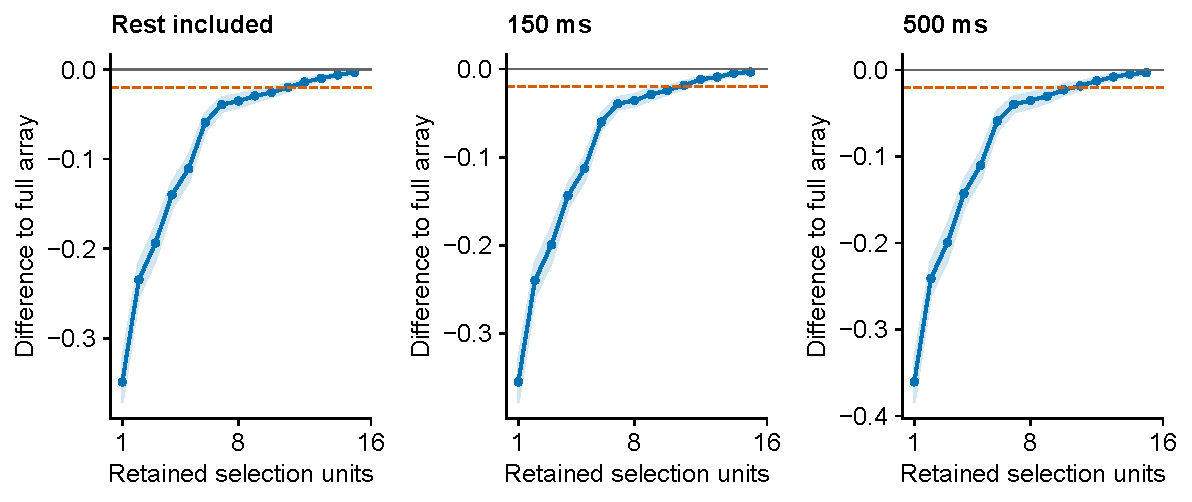
\includegraphics[width=\textwidth]{../figures/vector/figS1_sensitivity_curves.pdf}
\caption{Complete sensitivity curves for rest inclusion and alternate window lengths. Each mean paired change compares with full16 under that condition. Shading is a 95\% participant-bootstrap interval; dashed lines mark the 0.02 tolerance. Rankings are held at their primary 250 ms values.}\end{figure}
\begin{figure}[htbp]\centering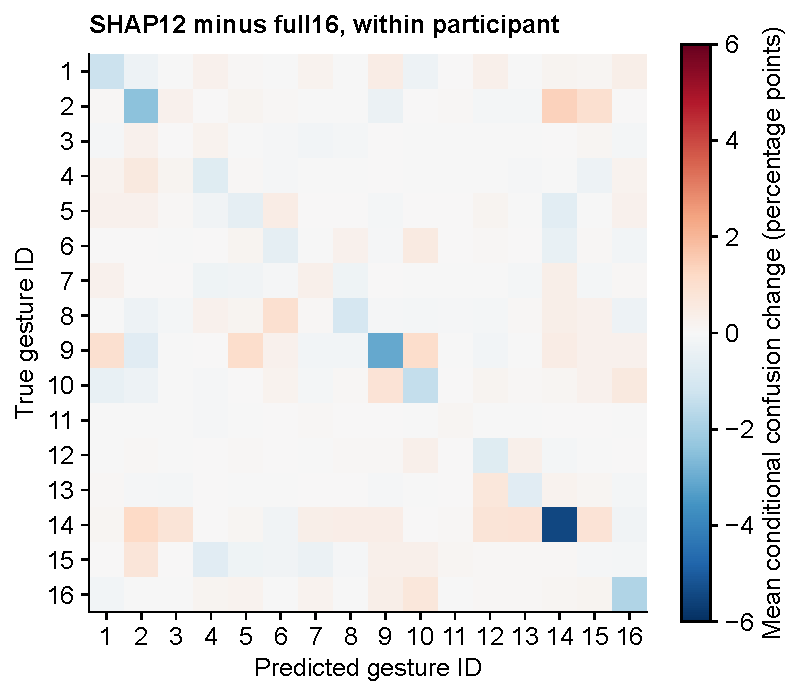
\includegraphics[width=.8\textwidth]{../figures/vector/figS2_confusion_change.pdf}
\caption{SHAP12 minus full16 confusion change. Each participant's confusion matrix is normalized within true gesture before averaging. The color scale is in percentage points, with symmetric limits covering the observed changes; machine-readable values retain full precision. Off-diagonal increases identify specific additional confusions without supplying independent window-level inference.}\end{figure}
\begin{figure}[htbp]\centering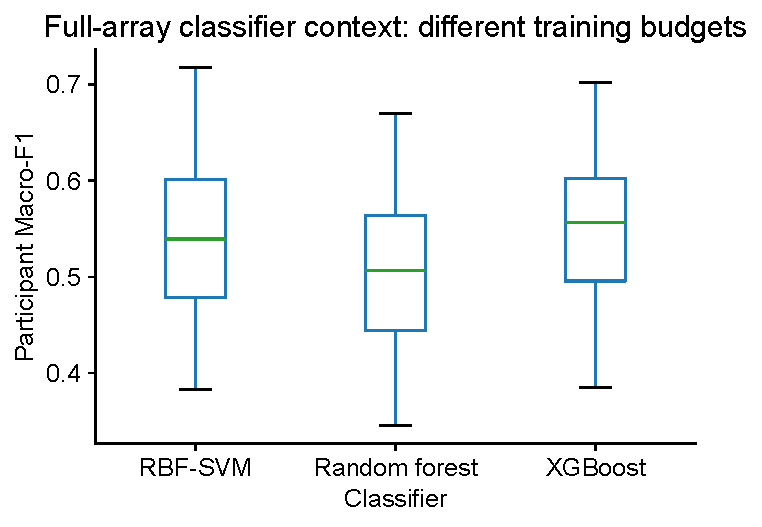
\includegraphics[width=.7\textwidth]{../figures/vector/figS3_classifier_context.pdf}
\caption{Full-array classifier comparison. Boxes summarize held-out participant Macro-F1. XGBoost uses all outer-training windows, random forest 200,000 and SVM 40,000; unequal budgets and budget calibration limit a direct classifier-capacity comparison. This is separate from the primary count curve's full16 reference.}\end{figure}
\begin{figure}[htbp]\centering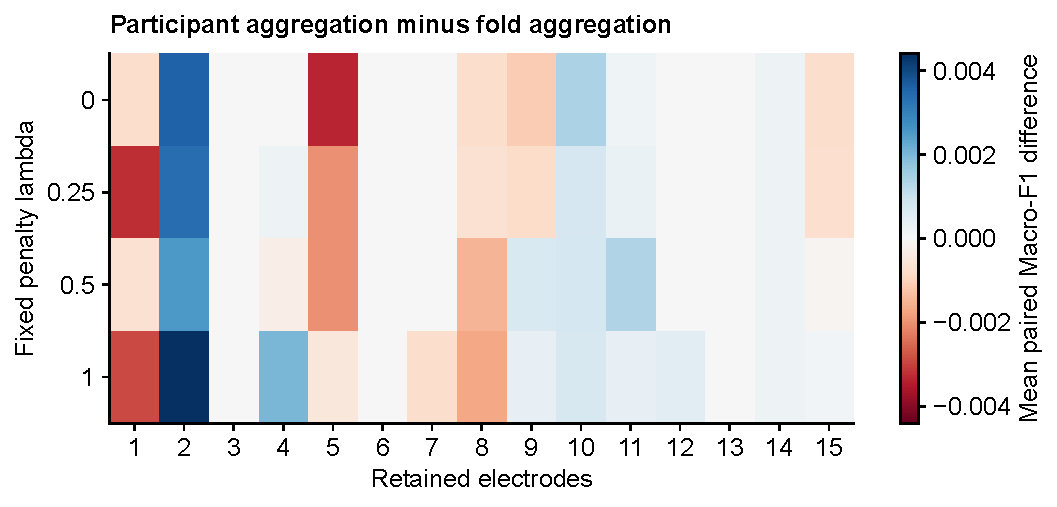
\includegraphics[width=\textwidth]{../figures/vector/figS4_participant_aggregation.pdf}
\caption{All participant-versus-fold aggregation comparisons. Each cell is the mean paired Macro-F1 change for one fixed penalty and count. The inferential family comprises sixty paired signed-rank comparisons with Holm adjustment. Colors use a symmetric difference scale; no penalty is selected from these outcomes.}\end{figure}
\begin{figure}[htbp]\centering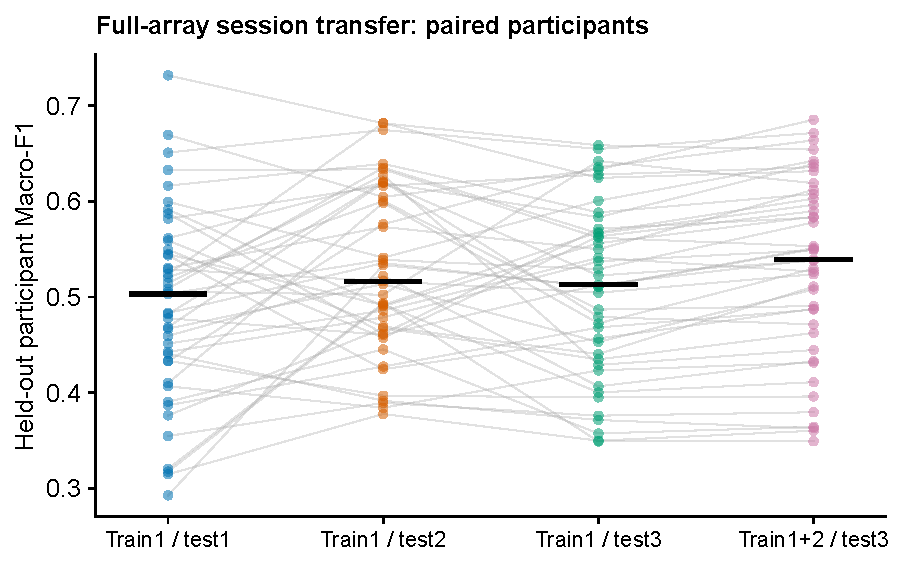
\includegraphics[width=.85\textwidth]{../figures/vector/figS5_cross_session.pdf}
\caption{Full-array session transfer for all held-out participants. Grey lines connect the same participant; colored points are observed scores and black bars are medians. Training on two sessions uses more observations, so the final contrast confounds session diversity and quantity. These are subject-independent full-array comparisons, not reduced-layout or isolated electrode-displacement tests.}\end{figure}
\begin{figure}[htbp]\centering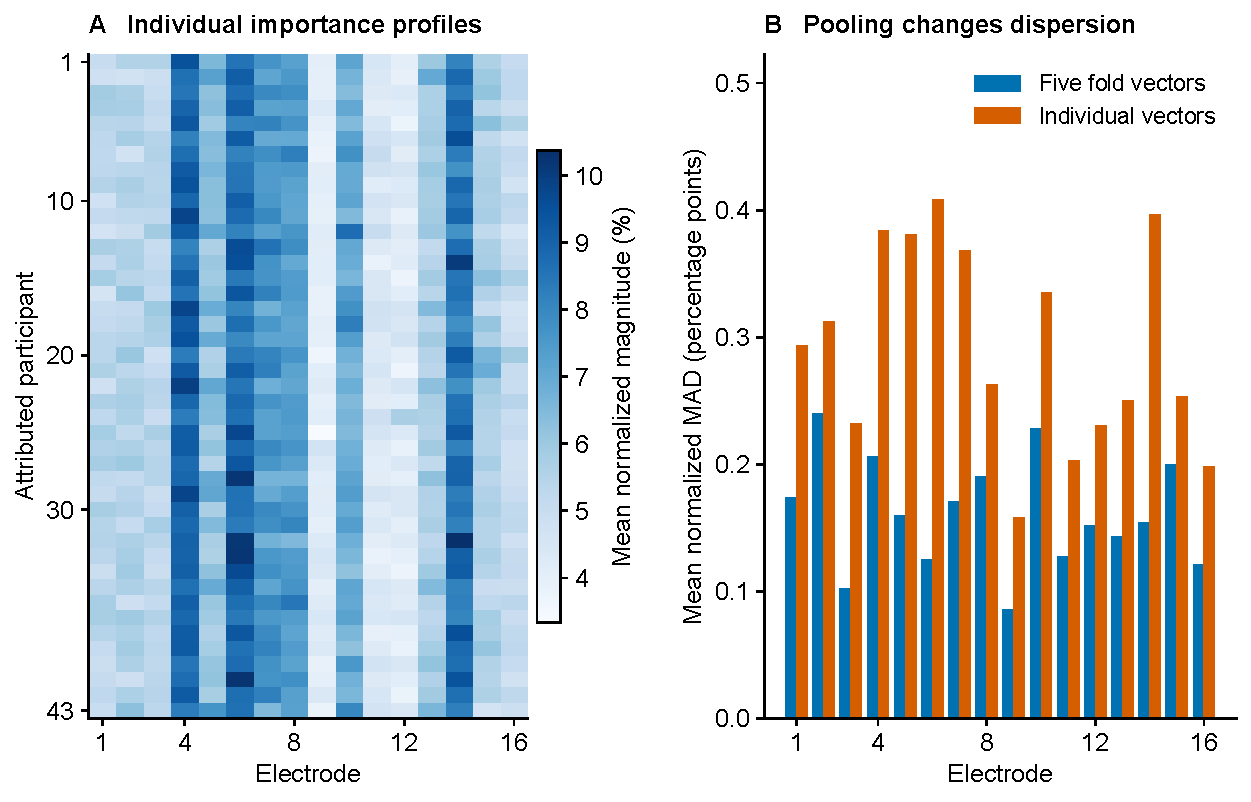
\includegraphics[width=\textwidth]{../figures/vector/figS6_attribution_heterogeneity.pdf}
\caption{Descriptive attribution heterogeneity. (A) Each participant's normalized profile averaged over outer-fold attribution records. (B) Mean MAD per electrode from five pooled inner-fold vectors versus individual participant vectors. These aggregates share fitted models and overlapping training cohorts; neither cells nor vectors are independent statistical replicates. Larger person dispersion does not imply a beneficial performance penalty.}\end{figure}
\begin{figure}[htbp]\centering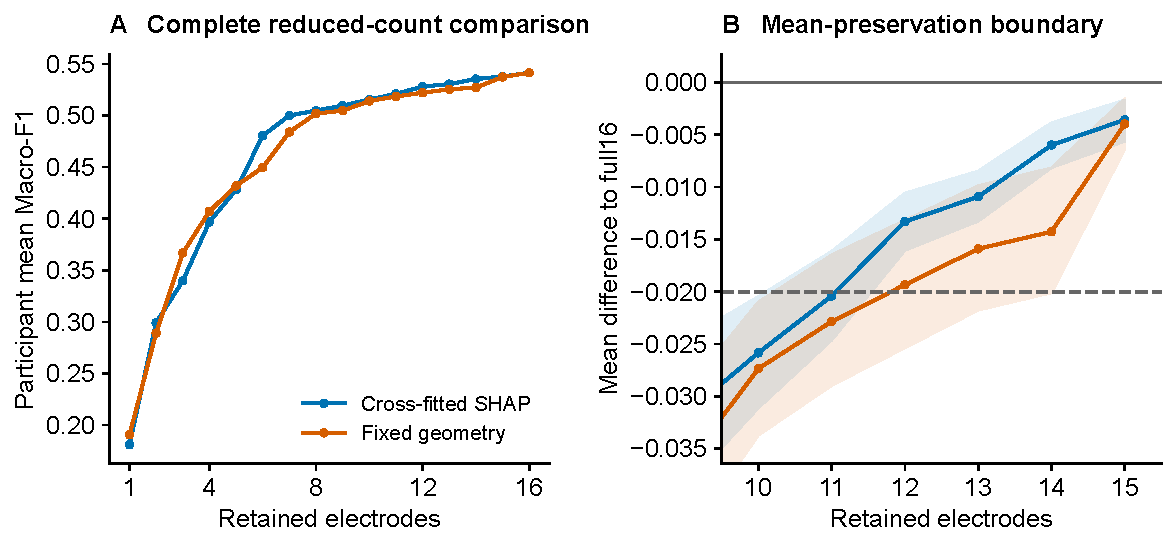
\includegraphics[width=\textwidth]{../figures/vector/figS7_geometric_count_curve.pdf}
\caption{Complete reduced-count comparison under the primary protocol. SHAP and the fixed geometric ordering use the same training sample and common full16 reference. The left panel includes every reduced count; the right enlarges the tolerance region. Shading gives participant-bootstrap intervals and the dashed line is the 0.02 margin. Different minimum qualifying counts do not establish a direct between-method mean difference.}\label{fig:geometricfull}\end{figure}
\FloatBarrier\clearpage
\section{Result tables}
\begin{table}[htbp]
\centering
\small
\caption{Full-array (16-electrode) leave-one-subject-out performance of three classifiers on GRABMyo (43 participants, 16 active gestures). CI: 95\% participant cluster-bootstrap confidence interval. RBF-SVM: support vector machine with a radial basis function kernel. Training windows: windows used to fit each fold's model.}
\label{tab:full_channel}
\setlength{\tabcolsep}{4pt}
\begin{adjustbox}{max width=\textwidth}
\begin{tabular}{llcccc}
\toprule
Model & Training windows & Macro-F1 & 95\% CI & SD & Range \\
\midrule
XGBoost & all (550{,}368 per fold) & 0.542 & 0.517--0.567 & 0.085 & 0.385--0.702 \\
RBF-SVM & 40{,}000 & 0.538 & 0.513--0.562 & 0.085 & 0.383--0.718 \\
Random forest & 200{,}000 & 0.502 & 0.475--0.528 & 0.090 & 0.346--0.670 \\
\bottomrule
\end{tabular}
\end{adjustbox}
\par\smallskip\parbox{0.95\linewidth}{\footnotesize Paired comparisons (Wilcoxon signed-rank, Holm over 3): Random forest $-$ RBF-SVM = $-$0.0362 (95\% CI $-$0.0444 to $-$0.0284), $p_{\mathrm{Holm}}$ $<$ 0.001, $r_{rb}$ = $-$0.97; Random forest $-$ XGBoost = $-$0.0408 (95\% CI $-$0.0475 to $-$0.0340), $p_{\mathrm{Holm}}$ $<$ 0.001, $r_{rb}$ = $-$0.98; RBF-SVM $-$ XGBoost = $-$0.0045 (95\% CI $-$0.0107 to +0.0015), $p_{\mathrm{Holm}}$ = 0.154, $r_{rb}$ = $-$0.25.}
\end{table}

\begin{table}[htbp]
\centering
\small
\caption{Electrode-count performance curve and primary non-inferiority decision on GRABMyo (cross-fitted ranking, $\lambda = 0$; 43 participants; every $k$ retrained from scratch on the same 200,000 training windows of each fold). $\Delta_k$: mean paired difference from the $k = 16$ model of the same curve, with 95\% participant cluster-bootstrap confidence interval (CI). Non-inferior: lower bound above $-\delta$ with the primary margin $\delta = 0.02$; Holm: the percentile-tail calculation with Holm correction over the 15 subset sizes; this is not a null-generated test. The smallest non-inferior subset ($k^*$) is in bold; the rule below it marks the boundary. Decisions at the sensitivity margins $\delta = 0.01$ and 0.03 are given in the count-inference comparison table.}
\label{tab:sparse_ni}
\setlength{\tabcolsep}{4pt}
\begin{adjustbox}{max width=\textwidth}
\begin{tabular}{rccccc}
\toprule
$k$ & Macro-F1 (mean $\pm$ SD) & $\Delta_k$ & 95\% CI & Non-inferior & Non-inferior (Holm) \\
\midrule
16 & 0.541 $\pm$ 0.084 & reference &  &  &  \\
15 & 0.538 $\pm$ 0.083 & $-$0.0036 & $-$0.0056 to $-$0.0017 & yes & yes \\
14 & 0.535 $\pm$ 0.083 & $-$0.0060 & $-$0.0081 to $-$0.0039 & yes & yes \\
13 & 0.530 $\pm$ 0.083 & $-$0.0109 & $-$0.0133 to $-$0.0085 & yes & yes \\
\textbf{12} & \textbf{0.528 $\pm$ 0.084} & \textbf{$-$0.0133} & \textbf{$-$0.0160 to $-$0.0106} & \textbf{yes} & \textbf{yes} \\
\midrule 11 & 0.521 $\pm$ 0.084 & $-$0.0204 & $-$0.0246 to $-$0.0162 & no & no \\
10 & 0.515 $\pm$ 0.083 & $-$0.0259 & $-$0.0311 to $-$0.0205 & no & no \\
9 & 0.510 $\pm$ 0.086 & $-$0.0318 & $-$0.0387 to $-$0.0246 & no & no \\
8 & 0.505 $\pm$ 0.085 & $-$0.0366 & $-$0.0440 to $-$0.0289 & no & no \\
7 & 0.500 $\pm$ 0.085 & $-$0.0413 & $-$0.0489 to $-$0.0333 & no & no \\
6 & 0.480 $\pm$ 0.084 & $-$0.0610 & $-$0.0713 to $-$0.0507 & no & no \\
5 & 0.428 $\pm$ 0.075 & $-$0.1133 & $-$0.1277 to $-$0.0993 & no & no \\
4 & 0.397 $\pm$ 0.071 & $-$0.1444 & $-$0.1590 to $-$0.1306 & no & no \\
3 & 0.340 $\pm$ 0.057 & $-$0.2015 & $-$0.2212 to $-$0.1822 & no & no \\
2 & 0.299 $\pm$ 0.057 & $-$0.2420 & $-$0.2603 to $-$0.2230 & no & no \\
1 & 0.181 $\pm$ 0.040 & $-$0.3603 & $-$0.3832 to $-$0.3369 & no & no \\
\bottomrule
\end{tabular}
\end{adjustbox}
\end{table}

\begin{table}[htbp]
\centering
\small
\caption{H2: attribution-ranked subsets versus the mean of random subsets of the same size (GRABMyo, 43 participants; post-hoc secondary family of 8 tests, Holm-corrected). All subsets were evaluated with one comparison model (XGBoost, 50 boosting rounds, 150,000 training windows per fold), these scores use a different protocol from table~\ref{tab:sparse_ni}. Random: participant's mean over 100 random subsets (500 at $k = 12$). Difference: mean paired difference (attribution minus random) with 95\% participant cluster-bootstrap confidence interval (CI). Higher/lower: participants for whom the attribution subset scored above/below their random mean. $p_{\mathrm{Holm}}$: Wilcoxon signed-rank, Holm-corrected; $r_{rb}$: matched-pairs rank-biserial correlation.}
\label{tab:h2}
\setlength{\tabcolsep}{4pt}
\begin{adjustbox}{max width=\textwidth}
\begin{tabular}{rlccccccc}
\toprule
$k$ & Ranking & Attribution & Random & Difference & 95\% CI & Higher/lower & $p_{\mathrm{Holm}}$ & $r_{rb}$ \\
\midrule
4 & Cross-fitted SHAP ($\lambda = 0$) & 0.382 & 0.366 & +0.0163 & +0.0060 to +0.0267 & 29/14 & 0.007 & +0.47 \\
 & Penalized SHAP ($\lambda = 0.5$) & 0.383 & 0.366 & +0.0172 & +0.0071 to +0.0274 & 30/13 & 0.007 & +0.50 \\
\midrule 6 & Cross-fitted SHAP ($\lambda = 0$) & 0.453 & 0.416 & +0.0370 & +0.0286 to +0.0452 & 37/6 & $<$0.001 & +0.92 \\
 & Penalized SHAP ($\lambda = 0.5$) & 0.453 & 0.416 & +0.0370 & +0.0286 to +0.0452 & 37/6 & $<$0.001 & +0.92 \\
\midrule 8 & Cross-fitted SHAP ($\lambda = 0$) & 0.468 & 0.445 & +0.0230 & +0.0161 to +0.0298 & 36/7 & $<$0.001 & +0.82 \\
 & Penalized SHAP ($\lambda = 0.5$) & 0.469 & 0.445 & +0.0243 & +0.0176 to +0.0308 & 37/6 & $<$0.001 & +0.86 \\
\midrule 12 & Cross-fitted SHAP ($\lambda = 0$) & 0.485 & 0.478 & +0.0074 & +0.0046 to +0.0103 & 35/8 & $<$0.001 & +0.71 \\
 & Penalized SHAP ($\lambda = 0.5$) & 0.485 & 0.478 & +0.0074 & +0.0046 to +0.0103 & 35/8 & $<$0.001 & +0.71 \\
\bottomrule
\end{tabular}
\end{adjustbox}
\end{table}

\begin{table}[htbp]
\centering
\small
\caption{H3: stability-regularised ranking ($\lambda > 0$) minus magnitude-only ranking ($\lambda = 0$) on the electrode-count performance curve (GRABMyo, 43 participants). Mean paired difference with 95\% participant cluster-bootstrap confidence interval (CI). Tied: participants for whom both rankings select the identical subset. $p_{\mathrm{Holm}}$: Wilcoxon signed-rank, Holm over 12 tests. $r_{rb}$ is computed from untied participants only and is undefined (--) when all are tied; with most participants tied it is not informative about magnitude.}
\label{tab:lambda}
\setlength{\tabcolsep}{4pt}
\begin{adjustbox}{max width=\textwidth}
\begin{tabular}{rrccccc}
\toprule
$\lambda$ & $k$ & Mean difference & 95\% CI & Tied & $p_{\mathrm{Holm}}$ & $r_{rb}$ \\
\midrule
0.25 & 4 & $-$0.0002 & $-$0.0005 to +0.0000 & 41/43 & 1.000 & $-$1.00 \\
0.25 & 6 & +0.0000 & +0.0000 to +0.0000 & 43/43 & 1.000 & -- \\
0.25 & 8 & +0.0001 & +0.0000 to +0.0002 & 42/43 & 1.000 & +1.00 \\
0.25 & 12 & +0.0000 & +0.0000 to +0.0000 & 43/43 & 1.000 & -- \\
0.5 & 4 & +0.0004 & $-$0.0005 to +0.0018 & 40/43 & 1.000 & +0.00 \\
0.5 & 6 & +0.0000 & +0.0000 to +0.0000 & 43/43 & 1.000 & -- \\
0.5 & 8 & +0.0008 & +0.0000 to +0.0019 & 40/43 & 1.000 & +1.00 \\
0.5 & 12 & +0.0000 & +0.0000 to +0.0000 & 43/43 & 1.000 & -- \\
1 & 4 & +0.0010 & $-$0.0003 to +0.0027 & 38/43 & 1.000 & +0.47 \\
1 & 6 & +0.0000 & +0.0000 to +0.0000 & 43/43 & 1.000 & -- \\
1 & 8 & +0.0015 & +0.0004 to +0.0028 & 36/43 & 0.216 & +1.00 \\
1 & 12 & $-$0.0005 & $-$0.0014 to +0.0000 & 42/43 & 1.000 & $-$1.00 \\
\bottomrule
\end{tabular}
\end{adjustbox}
\end{table}

\begin{table}[htbp]
\centering
\small
\caption{H4: deletion with retraining (GRABMyo, 43 participants). Retained: electrodes kept after deletion. Remove-Top, Remove-Bottom and Remove-Random delete the highest-ranked, lowest-ranked or randomly chosen electrodes; Remove-Random uses the random subsets of the H2 comparison and exists only where these were sampled. All orders use the same comparison model and training sample. Difference: mean paired difference (first minus second order) with 95\% participant cluster-bootstrap confidence interval (CI); negative values follow the expected ordering. $p_{\mathrm{Holm}}$: Wilcoxon signed-rank, Holm over the 15 contrasts; $r_{rb}$: matched-pairs rank-biserial correlation.}
\label{tab:faithfulness}
\setlength{\tabcolsep}{4pt}
\begin{adjustbox}{max width=\textwidth}
\begin{tabular}{rlcccccc}
\toprule
Retained & Contrast & First & Second & Difference & 95\% CI & $p_{\mathrm{Holm}}$ & $r_{rb}$ \\
\midrule
2 & Top $-$ Bottom & 0.263 & 0.292 & $-$0.0297 & $-$0.0419 to $-$0.0166 & $<$0.001 & $-$0.67 \\
\midrule 4 & Top $-$ Bottom & 0.351 & 0.382 & $-$0.0314 & $-$0.0447 to $-$0.0177 & $<$0.001 & $-$0.64 \\
 & Top $-$ Random & 0.351 & 0.366 & $-$0.0151 & $-$0.0239 to $-$0.0061 & 0.010 & $-$0.51 \\
 & Random $-$ Bottom & 0.366 & 0.382 & $-$0.0163 & $-$0.0265 to $-$0.0061 & 0.013 & $-$0.47 \\
\midrule 6 & Top $-$ Bottom & 0.376 & 0.454 & $-$0.0775 & $-$0.0921 to $-$0.0627 & $<$0.001 & $-$0.96 \\
 & Top $-$ Random & 0.376 & 0.416 & $-$0.0398 & $-$0.0487 to $-$0.0307 & $<$0.001 & $-$0.91 \\
 & Random $-$ Bottom & 0.416 & 0.454 & $-$0.0377 & $-$0.0459 to $-$0.0293 & $<$0.001 & $-$0.93 \\
\midrule 8 & Top $-$ Bottom & 0.408 & 0.469 & $-$0.0618 & $-$0.0772 to $-$0.0461 & $<$0.001 & $-$0.89 \\
 & Top $-$ Random & 0.408 & 0.445 & $-$0.0377 & $-$0.0476 to $-$0.0273 & $<$0.001 & $-$0.86 \\
 & Random $-$ Bottom & 0.445 & 0.469 & $-$0.0242 & $-$0.0309 to $-$0.0172 & $<$0.001 & $-$0.86 \\
\midrule 10 & Top $-$ Bottom & 0.445 & 0.475 & $-$0.0297 & $-$0.0399 to $-$0.0188 & $<$0.001 & $-$0.73 \\
\midrule 12 & Top $-$ Bottom & 0.455 & 0.485 & $-$0.0302 & $-$0.0385 to $-$0.0218 & $<$0.001 & $-$0.84 \\
 & Top $-$ Random & 0.455 & 0.478 & $-$0.0228 & $-$0.0296 to $-$0.0158 & $<$0.001 & $-$0.81 \\
 & Random $-$ Bottom & 0.478 & 0.485 & $-$0.0074 & $-$0.0101 to $-$0.0046 & $<$0.001 & $-$0.74 \\
\midrule 14 & Top $-$ Bottom & 0.487 & 0.491 & $-$0.0038 & $-$0.0084 to +0.0009 & 0.150 & $-$0.25 \\
\bottomrule
\end{tabular}
\end{adjustbox}
\end{table}

\begin{table}[htbp]
\centering
\small
\caption{Agreement of electrode rankings on GRABMyo ($\lambda = 0$). Values are mean (SD) over all pairs of rankings in each group. They are descriptive summaries: pairwise observations share rankings and are not independent, so no inferential interval is given.}
\label{tab:stability}
\setlength{\tabcolsep}{4pt}
\begin{adjustbox}{max width=\textwidth}
\begin{tabular}{lcccccc}
\toprule
Rankings compared & Pairs & Spearman $\rho$ & Kendall $\tau$ & Jaccard, top 4 & Jaccard, top 6 & Jaccard, top 8 \\
\midrule
Individual participants & 903 & 0.927 (0.038) & 0.801 (0.066) & 0.752 (0.194) & 0.905 (0.137) & 0.803 (0.132) \\
Inner folds (disjoint participant groups) & 430 & 0.948 (0.021) & 0.840 (0.046) & 0.816 (0.200) & 0.992 (0.047) & 0.838 (0.105) \\
Outer folds (overlapping training sets$^*$) & 903 & 0.987 (0.008) & 0.943 (0.028) & 0.888 (0.180) & 1.000 (0.000) & 0.923 (0.106) \\
\bottomrule
\end{tabular}
\end{adjustbox}
\par\smallskip\parbox{0.95\linewidth}{\footnotesize $^*$Outer training sets share about 98\% of their participants, so their agreement is descriptive only and is not an estimate of between-participant stability.}
\end{table}

\begin{table}[htbp]
\centering
\small
\caption{NinaPro DB5 channel-count performance curve (exploratory replication; cross-fitted ranking, $\lambda = 0$; 10 subjects; reference $k = 16$, mean Macro-F1 0.281; margin $\delta = 0.02$). The lower 95\% bound is shown to six decimals because the $k = 12$ decision lies at the margin. Non-inferior: lower bound above $-\delta$, unadjusted and under percentile-tail Holm correction over 15 subset sizes. Monte Carlo repetitions: number of 200 bootstrap repetitions in which the unadjusted decision was non-inferior. This is a Monte Carlo decision-stability diagnostic, not a probability that the hypothesis is true.}
\label{tab:replication}
\setlength{\tabcolsep}{4pt}
\begin{adjustbox}{max width=\textwidth}
\begin{tabular}{rcccccc}
\toprule
$k$ & Macro-F1 & $\Delta_k$ & Lower bound & Non-inf. & Non-inf. (Holm) & \makecell{Qualifying\\repetitions} \\
\midrule
15 & 0.270 & $-$0.0108 & $-$0.023773 & no & no & 0/200 (0.0\%) \\
14 & 0.269 & $-$0.0119 & $-$0.027438 & no & no & 0/200 (0.0\%) \\
13 & 0.266 & $-$0.0143 & $-$0.031186 & no & no & 0/200 (0.0\%) \\
12 & 0.268 & $-$0.0126 & $-$0.019994 & yes & no & 191/200 (95.5\%) \\
11 & 0.260 & $-$0.0211 & $-$0.034121 & no & no & 0/200 (0.0\%) \\
10 & 0.265 & $-$0.0160 & $-$0.031368 & no & no & 0/200 (0.0\%) \\
9 & 0.260 & $-$0.0202 & $-$0.036943 & no & no & 0/200 (0.0\%) \\
8 & 0.252 & $-$0.0288 & $-$0.055369 & no & no & 0/200 (0.0\%) \\
7 & 0.232 & $-$0.0486 & $-$0.075346 & no & no & 0/200 (0.0\%) \\
6 & 0.231 & $-$0.0498 & $-$0.081816 & no & no & 0/200 (0.0\%) \\
5 & 0.200 & $-$0.0803 & $-$0.118422 & no & no & 0/200 (0.0\%) \\
4 & 0.180 & $-$0.1006 & $-$0.150266 & no & no & 0/200 (0.0\%) \\
3 & 0.162 & $-$0.1185 & $-$0.174145 & no & no & 0/200 (0.0\%) \\
2 & 0.138 & $-$0.1430 & $-$0.195307 & no & no & 0/200 (0.0\%) \\
1 & 0.105 & $-$0.1754 & $-$0.229548 & no & no & 0/200 (0.0\%) \\
\bottomrule
\end{tabular}
\end{adjustbox}
\end{table}

\begin{table}[htbp]
\centering
\small
\caption{Cross-session evaluation on GRABMyo (exploratory; full array). All conditions are also subject-independent: the test participant is never in training.}
\label{tab:cross_session}
\setlength{\tabcolsep}{4pt}
\begin{adjustbox}{max width=\textwidth}
\begin{tabular}{lcccc}
\toprule
Design & Train sessions & Test session & Train windows & Macro-F1 \\
\midrule
CS1 & 1 & 1 & 183{,}456 & 0.492 $\pm$ 0.101 \\
CS1 & 1 & 2 & 183{,}456 & 0.528 $\pm$ 0.088 \\
CS1 & 1 & 3 & 183{,}456 & 0.510 $\pm$ 0.090 \\
CS2 & 1+2 & 3 & 366{,}912 & 0.530 $\pm$ 0.095 \\
\bottomrule
\end{tabular}
\end{adjustbox}
\par\smallskip\parbox{0.95\linewidth}{\footnotesize Paired contrasts (exploratory, uncorrected): CS1: test S2 $-$ test S1: +0.0355 (95\% CI +0.0091 to +0.0621), $p$ = 0.024; CS1: test S3 $-$ test S1: +0.0172 (95\% CI $-$0.0038 to +0.0391), $p$ = 0.272; S3 test: CS2 (train S1+S2) $-$ CS1 (train S1): +0.0210 (95\% CI +0.0146 to +0.0274), $p$ $<$ 0.001.}
\end{table}

\begin{table}[htbp]
\centering
\small
\caption{GRABMyo derived bipolar pairs $F_j - F_{j+8}$ (exploratory; 43 participants; $\lambda = 0$; count-feature threshold $4 \times 10^{-3}$~mV; margin $\delta = 0.02$). Reference: the $k = 8$ model of the same curve, trained on the curve's 200,000-window sample (mean Macro-F1 0.480). An additional full-array bipolar value (0.478) comes from a separate model trained on all 550{,}368 training windows of each fold, as for the monopolar analysis. $\Delta_k$: mean paired difference with 95\% participant cluster-bootstrap confidence interval (CI). Monte Carlo repetitions: as in the DB5 table in this Supplementary.}
\label{tab:bipolar}
\setlength{\tabcolsep}{4pt}
\begin{adjustbox}{max width=\textwidth}
\begin{tabular}{rccccc}
\toprule
$k$ & Macro-F1 & $\Delta_k$ & 95\% CI & Non-inf. & \makecell{Qualifying\\repetitions} \\
\midrule
7 & 0.464 & $-$0.0158 & $-$0.0203 to $-$0.0113 & no & 0/200 (0.0\%) \\
6 & 0.442 & $-$0.0375 & $-$0.0451 to $-$0.0303 & no & 0/200 (0.0\%) \\
5 & 0.405 & $-$0.0742 & $-$0.0845 to $-$0.0646 & no & 0/200 (0.0\%) \\
4 & 0.356 & $-$0.1240 & $-$0.1392 to $-$0.1096 & no & 0/200 (0.0\%) \\
3 & 0.310 & $-$0.1697 & $-$0.1852 to $-$0.1546 & no & 0/200 (0.0\%) \\
2 & 0.240 & $-$0.2399 & $-$0.2615 to $-$0.2177 & no & 0/200 (0.0\%) \\
1 & 0.174 & $-$0.3052 & $-$0.3298 to $-$0.2790 & no & 0/200 (0.0\%) \\
\bottomrule
\end{tabular}
\end{adjustbox}
\end{table}

\begin{table}[htbp]
\centering\small
\caption{Paired participant-level gesture F1: SHAP12 minus full16, with Holm correction across all sixteen active gestures. Numeric IDs follow the dataset MotionSequence.txt, reproduced in the gesture dictionary.}\label{tab:gesture}
\begin{adjustbox}{max width=\textwidth}
\begin{tabular}{llllll}\toprule
Gesture ID & Full16 & SHAP12 & $\bar\Delta$ & 95\% CI & $p_{\rm Holm}$\\\midrule
1 & 0.449 & 0.437 & -0.0119 & [-0.0210, -0.0035] & 0.086\\
2 & 0.308 & 0.284 & -0.0242 & [-0.0356, -0.0132] & 0.003\\
3 & 0.519 & 0.516 & -0.0030 & [-0.0117, +0.0054] & 1.000\\
4 & 0.348 & 0.341 & -0.0069 & [-0.0137, -0.0001] & 0.121\\
5 & 0.490 & 0.483 & -0.0066 & [-0.0176, +0.0045] & 1.000\\
6 & 0.604 & 0.592 & -0.0115 & [-0.0222, -0.0008] & 0.133\\
7 & 0.503 & 0.504 & +0.0009 & [-0.0059, +0.0083] & 1.000\\
8 & 0.499 & 0.489 & -0.0099 & [-0.0215, +0.0006] & 0.787\\
9 & 0.387 & 0.357 & -0.0300 & [-0.0436, -0.0167] & 0.002\\
10 & 0.533 & 0.514 & -0.0192 & [-0.0299, -0.0094] & 0.005\\
11 & 0.940 & 0.939 & -0.0003 & [-0.0018, +0.0012] & 1.000\\
12 & 0.830 & 0.819 & -0.0107 & [-0.0202, -0.0014] & 0.079\\
13 & 0.813 & 0.804 & -0.0093 & [-0.0156, -0.0036] & 0.085\\
14 & 0.487 & 0.441 & -0.0456 & [-0.0594, -0.0323] & $<0.001$\\
15 & 0.543 & 0.536 & -0.0066 & [-0.0142, +0.0014] & 0.168\\
16 & 0.410 & 0.392 & -0.0179 & [-0.0322, -0.0034] & 0.168\\
\bottomrule\end{tabular}
\end{adjustbox}
\end{table}

\begin{table}[htbp]
\centering\small
\caption{Participant-level minus fold aggregation at count 12. Holm adjustment covers all sixty reduced-count comparisons across four penalties; full results are in the paired-comparison CSV.}\label{tab:personextension}
\begin{adjustbox}{max width=\textwidth}
\begin{tabular}{lllll}\toprule
$\lambda$ & $k$ & $\bar\Delta$ & 95\% CI & $p_{\rm Holm}$\\\midrule
0.0 & 12 & +0.0000 & [+0.0000, +0.0000] & 1.000\\
0.25 & 12 & +0.0000 & [+0.0000, +0.0000] & 1.000\\
0.5 & 12 & +0.0000 & [+0.0000, +0.0000] & 1.000\\
1.0 & 12 & +0.0005 & [+0.0000, +0.0014] & 1.000\\
\bottomrule\end{tabular}
\end{adjustbox}
\end{table}

\begin{table}[htbp]
\centering\small
\caption{Participant aggregation: penalized minus unpenalized attribution. Holm correction covers all twelve tests; all fixed penalty settings are reported.}\label{tab:penalty}
\begin{adjustbox}{max width=\textwidth}
\begin{tabular}{lllll}\toprule
$\lambda$ & $k$ & $\bar\Delta$ & 95\% CI & $p_{\rm Holm}$\\\midrule
0.25 & 4 & +0.0000 & [+0.0000, +0.0000] & 1.000\\
0.25 & 6 & +0.0000 & [+0.0000, +0.0000] & 1.000\\
0.25 & 8 & +0.0002 & [-0.0008, +0.0011] & 1.000\\
0.25 & 12 & +0.0000 & [+0.0000, +0.0000] & 1.000\\
0.5 & 4 & +0.0001 & [+0.0000, +0.0004] & 1.000\\
0.5 & 6 & +0.0000 & [+0.0000, +0.0000] & 1.000\\
0.5 & 8 & +0.0000 & [-0.0011, +0.0011] & 1.000\\
0.5 & 12 & +0.0000 & [+0.0000, +0.0000] & 1.000\\
1.0 & 4 & +0.0030 & [+0.0006, +0.0060] & 0.332\\
1.0 & 6 & +0.0000 & [+0.0000, +0.0000] & 1.000\\
1.0 & 8 & +0.0005 & [-0.0008, +0.0018] & 1.000\\
1.0 & 12 & +0.0000 & [+0.0000, +0.0000] & 1.000\\
\bottomrule\end{tabular}
\end{adjustbox}
\end{table}

\begin{table}[htbp]
\centering\small
\caption{Post-hoc descriptive selector activity: each fixed positive penalty versus its unpenalized counterpart. Counts concern physical site sets, not rank order. Every row includes all 43 participants; the CSV retains all sixteen counts. Identical site sets do not constitute an equivalence test of distinct layouts.}\label{tab:selectionchanges}
\begin{adjustbox}{max width=\textwidth}
\begin{tabular}{lllll}\toprule
Aggregation & $\lambda$ & $k$ & Changed sets & Mean Jaccard\\\midrule
Fold & 0.25 & 4 & 2/43 & 0.981\\
Fold & 0.25 & 6 & 0/43 & 1.000\\
Fold & 0.25 & 8 & 1/43 & 0.995\\
Fold & 0.25 & 12 & 0/43 & 1.000\\
Fold & 0.5 & 4 & 3/43 & 0.972\\
Fold & 0.5 & 6 & 0/43 & 1.000\\
Fold & 0.5 & 8 & 3/43 & 0.984\\
Fold & 0.5 & 12 & 0/43 & 1.000\\
Fold & 1.0 & 4 & 5/43 & 0.953\\
Fold & 1.0 & 6 & 0/43 & 1.000\\
Fold & 1.0 & 8 & 7/43 & 0.964\\
Fold & 1.0 & 12 & 1/43 & 0.996\\
Participant & 0.25 & 4 & 0/43 & 1.000\\
Participant & 0.25 & 6 & 0/43 & 1.000\\
Participant & 0.25 & 8 & 3/43 & 0.984\\
Participant & 0.25 & 12 & 0/43 & 1.000\\
Participant & 0.5 & 4 & 1/43 & 0.991\\
Participant & 0.5 & 6 & 0/43 & 1.000\\
Participant & 0.5 & 8 & 5/43 & 0.974\\
Participant & 0.5 & 12 & 0/43 & 1.000\\
Participant & 1.0 & 4 & 6/43 & 0.944\\
Participant & 1.0 & 6 & 0/43 & 1.000\\
Participant & 1.0 & 8 & 7/43 & 0.964\\
Participant & 1.0 & 12 & 0/43 & 1.000\\
\bottomrule\end{tabular}
\end{adjustbox}
\end{table}

\begin{table}[htbp]
\centering\small
\caption{Two exploratory split-derived layouts at twelve electrodes, fitted with all development windows. Six-decimal limits preserve the strict boundary decision. Layout estimation excludes test participants, but count selection had already used the full cohort. All penalties produced the same layout within each split.}\label{tab:fixedlayouts}
\begin{adjustbox}{max width=\textwidth}
\begin{tabular}{llllll}\toprule
Development / test & $n$ test & Dropped sites & $\bar\Delta$ & 95\% CI & NI\\\midrule
odd / even & 21 & 3, 9, 11, 12 & -0.0124 & [-0.017901, -0.007658] & yes\\
even / odd & 22 & 9, 11, 12, 13 & -0.0135 & [-0.020020, -0.006627] & no\\
\bottomrule\end{tabular}
\end{adjustbox}
\end{table}

\begin{table}[htbp]
\centering\small
\caption{Full fixed geometric ordering under the primary 300-round, 200,000-window protocol. Each count uses all 43 participants and the common primary full16 reference.  The count-family null test is exploratory and Holm-adjusted over fifteen reduced counts.}\label{tab:geometriccurve}
\begin{adjustbox}{max width=\textwidth}
\begin{tabular}{llllll}\toprule
$k$ & Mean F1 & $\bar\Delta$ & 95\% CI & NI CI & NI null Holm\\\midrule
1 & 0.191 & -0.3506 & [-0.3718, -0.3288] & no & no\\
2 & 0.289 & -0.2523 & [-0.2714, -0.2325] & no & no\\
3 & 0.367 & -0.1746 & [-0.1911, -0.1569] & no & no\\
4 & 0.407 & -0.1341 & [-0.1497, -0.1185] & no & no\\
5 & 0.432 & -0.1095 & [-0.1232, -0.0954] & no & no\\
6 & 0.450 & -0.0917 & [-0.1030, -0.0796] & no & no\\
7 & 0.484 & -0.0574 & [-0.0683, -0.0463] & no & no\\
8 & 0.502 & -0.0395 & [-0.0467, -0.0321] & no & no\\
9 & 0.505 & -0.0367 & [-0.0438, -0.0296] & no & no\\
10 & 0.514 & -0.0274 & [-0.0337, -0.0210] & no & no\\
11 & 0.518 & -0.0229 & [-0.0290, -0.0165] & no & no\\
12 & 0.522 & -0.0193 & [-0.0254, -0.0132] & no & no\\
13 & 0.525 & -0.0159 & [-0.0218, -0.0099] & no & no\\
14 & 0.527 & -0.0143 & [-0.0201, -0.0082] & no & no\\
15 & 0.537 & -0.0040 & [-0.0063, -0.0016] & yes & yes\\
\bottomrule\end{tabular}
\end{adjustbox}
\end{table}

\begin{table}[htbp]
\centering\small
\caption{Count decisions from the primary percentile rule, percentile-tail Holm calculation and exploratory null-centred studentized bootstrap. Inference uses participants; each condition and margin is its own count family.}\label{tab:countinference}
\begin{adjustbox}{max width=\textwidth}
\begin{tabular}{lllll}\toprule
Condition & Margin & Percentile CI & Tail Holm & Null-centred Holm\\\midrule
Derived bipolar & 0.01 & none & none & none\\
Derived bipolar & 0.02 & none & none & none\\
Derived bipolar & 0.03 & 7 & 7 & 7\\
NinaPro DB5 & 0.01 & none & none & none\\
NinaPro DB5 & 0.02 & 12 & none & none\\
NinaPro DB5 & 0.03 & 12 & 12 & none\\
Geometric & 0.01 & 15 & 15 & 15\\
Geometric & 0.02 & 15 & 15 & 15\\
Geometric & 0.03 & 11 & 12 & 12\\
Participant ($\lambda=0$) & 0.01 & 14 & 14 & 14\\
Participant ($\lambda=0$) & 0.02 & 12 & 12 & 12\\
Participant ($\lambda=0$) & 0.03 & 11 & 11 & 11\\
Participant ($\lambda=0.25$) & 0.01 & 14 & 14 & 14\\
Participant ($\lambda=0.25$) & 0.02 & 12 & 12 & 12\\
Participant ($\lambda=0.25$) & 0.03 & 11 & 11 & 11\\
Participant ($\lambda=0.5$) & 0.01 & 14 & 14 & 14\\
Participant ($\lambda=0.5$) & 0.02 & 12 & 12 & 12\\
Participant ($\lambda=0.5$) & 0.03 & 11 & 11 & 11\\
Participant ($\lambda=1$) & 0.01 & 14 & 14 & 14\\
Participant ($\lambda=1$) & 0.02 & 12 & 12 & 12\\
Participant ($\lambda=1$) & 0.03 & 11 & 11 & 11\\
Primary ($\lambda=0$) & 0.01 & 14 & 14 & 14\\
Primary ($\lambda=0$) & 0.02 & 12 & 12 & 12\\
Primary ($\lambda=0$) & 0.03 & 11 & 11 & 11\\
Rest included & 0.01 & 14 & 14 & 14\\
Rest included & 0.02 & 12 & 12 & 12\\
Rest included & 0.03 & 11 & 11 & 11\\
150 ms & 0.01 & 14 & 14 & 14\\
150 ms & 0.02 & 12 & 12 & 12\\
150 ms & 0.03 & 10 & 11 & 11\\
500 ms & 0.01 & 14 & 14 & 14\\
500 ms & 0.02 & 12 & 12 & 12\\
500 ms & 0.03 & 10 & 11 & 11\\
\bottomrule\end{tabular}
\end{adjustbox}
\end{table}

\begin{table}[htbp]
\centering\small
\caption{Observed resource-matched selection-stage runtime per outer fold on the recorded workstation. Inner training is shared and counted once. Measurements include concurrent workstation load and are descriptive rather than an isolated benchmark. No online or real-time latency is inferred.}\label{tab:costs}
\begin{adjustbox}{max width=\textwidth}
\begin{tabular}{lllll}\toprule
Stage & Mean s & SD s & Min s & Max s\\\midrule
Shared inner training & 117.1 & 3.7 & 114.7 & 136.4\\
TreeSHAP selection & 4.0 & 0.2 & 3.8 & 4.3\\
Grouped permutation & 10.6 & 1.1 & 9.8 & 13.3\\
\bottomrule\end{tabular}
\end{adjustbox}
\end{table}



\end{document}
